% Figura Anexo II: la función de consumo de la renta permanente (FRIEDMAN 1957): corto plazo plano, largo plazo proporcional
\documentclass[tikz,border=3pt]{standalone}
\usepackage[T1]{fontenc}
\usepackage[utf8]{inputenc}
\usetikzlibrary{arrows.meta,calc,positioning,decorations.pathreplacing}
\begin{document}
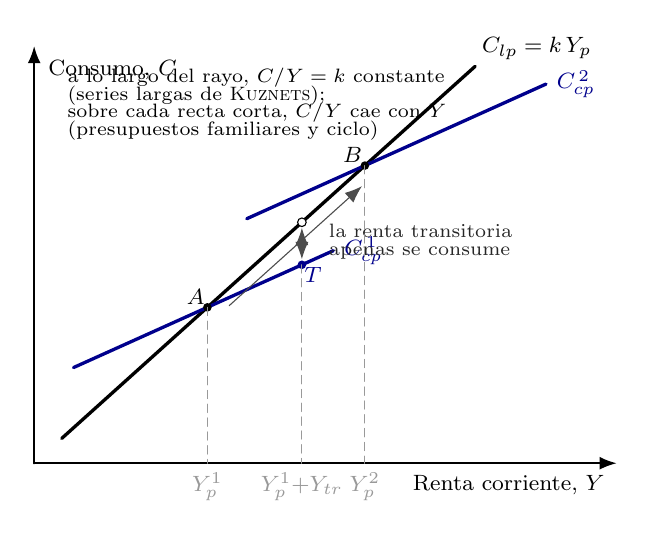
\begin{tikzpicture}[>={Latex[length=2.2mm]}, line cap=round, font=\footnotesize,
  eje/.style={->, thick},
  curva/.style={very thick},
  nueva/.style={very thick, blue!55!black},
  guia/.style={densely dashed, gray!80},
  pto/.style={circle, fill=black, inner sep=1.1pt}]
  \draw[eje] (0,0) -- (7.4,0) node[below left=1pt]{Renta corriente, $Y$};
  \draw[eje] (0,0) -- (0,5.3) node[below right=2pt]{Consumo, $C$};
  % Rayo de largo plazo C = k Y
  \draw[curva] (0.35,0.315) -- (5.6,5.04) node[above right=-2pt]{$C_{lp}=k\,Y_p$};
  % Rectas de corto plazo (dos periodos)
  \draw[nueva] (0.5,1.215) -- (3.8,2.70) node[right]{$C^{\,1}_{cp}$};
  \draw[nueva] (2.7,3.105) -- (6.5,4.815) node[right]{$C^{\,2}_{cp}$};
  % Puntos sobre el rayo (rentas medias = permanentes)
  \node[pto] (A) at (2.2,1.98) {};
  \node[above left=-2pt of A, inner sep=1pt] {$A$};
  \node[pto] (B) at (4.2,3.78) {};
  \node[above left=-2pt of B, inner sep=1pt] {$B$};
  % Punto con renta transitoria positiva
  \node[pto, fill=blue!55!black] (T) at (3.4,2.52) {};
  \node[below right=-2pt of T, inner sep=1pt, blue!55!black] {$T$};
  \node[circle, draw=black, fill=white, inner sep=1.1pt] (Tr) at (3.4,3.06) {};
  \draw[<->, gray!60!black, shorten >=2pt, shorten <=2pt] (3.4,3.06) -- (3.4,2.52);
  \node[align=left, anchor=west, gray!30!black] at (3.62,2.82) {\scriptsize la renta transitoria\\[-3pt]\scriptsize apenas se consume};
  % Guías
  \draw[guia] (2.2,1.98) -- (2.2,0) node[below]{$Y_p^{1}$};
  \draw[guia] (3.4,2.52) -- (3.4,0) node[below]{$Y_p^{1}{+}Y_{tr}$};
  \draw[guia] (4.2,3.78) -- (4.2,0) node[below]{$Y_p^{2}$};
  % Flecha secular
  \draw[->, gray!60!black, shorten >=6pt, shorten <=6pt] ($(A)+(0.12,-0.12)$) -- ($(B)+(0.12,-0.12)$);
  \node[align=left, anchor=north west] at (0.3,5.15) {\scriptsize a lo largo del rayo, $C/Y=k$ constante\\[-3pt]\scriptsize (series largas de \textsc{Kuznets});\\[-3pt]\scriptsize sobre cada recta corta, $C/Y$ cae con $Y$\\[-3pt]\scriptsize (presupuestos familiares y ciclo)};
\end{tikzpicture}
\end{document}
